%% bare_jrnl_transmag.tex
%% V1.4b
%% 2015/08/26
%% by Michael Shell
%% see http://www.michaelshell.org/
%% for current contact information.
%%
%% This is a skeleton file demonstrating the use of IEEEtran.cls
%% (requires IEEEtran.cls version 1.8b or later) with an IEEE 
%% Transactions on Magnetics journal paper.
%%
%% Support sites:
%% http://www.michaelshell.org/tex/ieeetran/
%% http://www.ctan.org/pkg/ieeetran
%% and
%% http://www.ieee.org/

%%*************************************************************************
%% Legal Notice:
%% This code is offered as-is without any warranty either expressed or
%% implied; without even the implied warranty of MERCHANTABILITY or
%% FITNESS FOR A PARTICULAR PURPOSE! 
%% User assumes all risk.
%% In no event shall the IEEE or any contributor to this code be liable for
%% any damages or losses, including, but not limited to, incidental,
%% consequential, or any other damages, resulting from the use or misuse
%% of any information contained here.
%%
%% All comments are the opinions of their respective authors and are not
%% necessarily endorsed by the IEEE.
%%
%% This work is distributed under the LaTeX Project Public License (LPPL)
%% ( http://www.latex-project.org/ ) version 1.3, and may be freely used,
%% distributed and modified. A copy of the LPPL, version 1.3, is included
%% in the base LaTeX documentation of all distributions of LaTeX released
%% 2003/12/01 or later.
%% Retain all contribution notices and credits.
%% ** Modified files should be clearly indicated as such, including  **
%% ** renaming them and changing author support contact information. **
%%*************************************************************************


% *** Authors should verify (and, if needed, correct) their LaTeX system  ***
% *** with the testflow diagnostic prior to trusting their LaTeX platform ***
% *** with production work. The IEEE's font choices and paper sizes can   ***
% *** trigger bugs that do not appear when using other class files.       ***                          ***
% The testflow support page is at:
% http://www.michaelshell.org/tex/testflow/



\documentclass[journal,transmag]{IEEEtran}
%
% If IEEEtran.cls has not been installed into the LaTeX system files,
% manually specify the path to it like:
% \documentclass[journal]{../sty/IEEEtran}





% Some very useful LaTeX packages include:
% (uncomment the ones you want to load)


% *** MISC UTILITY PACKAGES ***
%
%\usepackage{ifpdf}
% Heiko Oberdiek's ifpdf.sty is very useful if you need conditional
% compilation based on whether the output is pdf or dvi.
% usage:
% \ifpdf
%   % pdf code
% \else
%   % dvi code
% \fi
% The latest version of ifpdf.sty can be obtained from:
% http://www.ctan.org/pkg/ifpdf
% Also, note that IEEEtran.cls V1.7 and later provides a builtin
% \ifCLASSINFOpdf conditional that works the same way.
% When switching from latex to pdflatex and vice-versa, the compiler may
% have to be run twice to clear warning/error messages.






% *** CITATION PACKAGES ***
%
%\usepackage{cite}
% cite.sty was written by Donald Arseneau
% V1.6 and later of IEEEtran pre-defines the format of the cite.sty package
% \cite{} output to follow that of the IEEE. Loading the cite package will
% result in citation numbers being automatically sorted and properly
% "compressed/ranged". e.g., [1], [9], [2], [7], [5], [6] without using
% cite.sty will become [1], [2], [5]--[7], [9] using cite.sty. cite.sty's
% \cite will automatically add leading space, if needed. Use cite.sty's
% noadjust option (cite.sty V3.8 and later) if you want to turn this off
% such as if a citation ever needs to be enclosed in parenthesis.
% cite.sty is already installed on most LaTeX systems. Be sure and use
% version 5.0 (2009-03-20) and later if using hyperref.sty.
% The latest version can be obtained at:
% http://www.ctan.org/pkg/cite
% The documentation is contained in the cite.sty file itself.






% *** GRAPHICS RELATED PACKAGES ***
%
\ifCLASSINFOpdf
  % \usepackage[pdftex]{graphicx}
  % declare the path(s) where your graphic files are
  % \graphicspath{{../pdf/}{../jpeg/}}
  % and their extensions so you won't have to specify these with
  % every instance of \includegraphics
  % \DeclareGraphicsExtensions{.pdf,.jpeg,.png}
\else
  % or other class option (dvipsone, dvipdf, if not using dvips). graphicx
  % will default to the driver specified in the system graphics.cfg if no
  % driver is specified.
  % \usepackage[dvips]{graphicx}
  % declare the path(s) where your graphic files are
  % \graphicspath{{../eps/}}
  % and their extensions so you won't have to specify these with
  % every instance of \includegraphics
  % \DeclareGraphicsExtensions{.eps}
\fi
% graphicx was written by David Carlisle and Sebastian Rahtz. It is
% required if you want graphics, photos, etc. graphicx.sty is already
% installed on most LaTeX systems. The latest version and documentation
% can be obtained at: 
% http://www.ctan.org/pkg/graphicx
% Another good source of documentation is "Using Imported Graphics in
% LaTeX2e" by Keith Reckdahl which can be found at:
% http://www.ctan.org/pkg/epslatex
%
% latex, and pdflatex in dvi mode, support graphics in encapsulated
% postscript (.eps) format. pdflatex in pdf mode supports graphics
% in .pdf, .jpeg, .png and .mps (metapost) formats. Users should ensure
% that all non-photo figures use a vector format (.eps, .pdf, .mps) and
% not a bitmapped formats (.jpeg, .png). The IEEE frowns on bitmapped formats
% which can result in "jaggedy"/blurry rendering of lines and letters as
% well as large increases in file sizes.
%
% You can find documentation about the pdfTeX application at:
% http://www.tug.org/applications/pdftex




% *** MATH PACKAGES ***
%
%\usepackage{amsmath}
% A popular package from the American Mathematical Society that provides
% many useful and powerful commands for dealing with mathematics.
%
% Note that the amsmath package sets \interdisplaylinepenalty to 10000
% thus preventing page breaks from occurring within multiline equations. Use:
%\interdisplaylinepenalty=2500
% after loading amsmath to restore such page breaks as IEEEtran.cls normally
% does. amsmath.sty is already installed on most LaTeX systems. The latest
% version and documentation can be obtained at:
% http://www.ctan.org/pkg/amsmath





% *** SPECIALIZED LIST PACKAGES ***
%
%\usepackage{algorithmic}
% algorithmic.sty was written by Peter Williams and Rogerio Brito.
% This package provides an algorithmic environment fo describing algorithms.
% You can use the algorithmic environment in-text or within a figure
% environment to provide for a floating algorithm. Do NOT use the algorithm
% floating environment provided by algorithm.sty (by the same authors) or
% algorithm2e.sty (by Christophe Fiorio) as the IEEE does not use dedicated
% algorithm float types and packages that provide these will not provide
% correct IEEE style captions. The latest version and documentation of
% algorithmic.sty can be obtained at:
% http://www.ctan.org/pkg/algorithms
% Also of interest may be the (relatively newer and more customizable)
% algorithmicx.sty package by Szasz Janos:
% http://www.ctan.org/pkg/algorithmicx




% *** ALIGNMENT PACKAGES ***
%
%\usepackage{array}
% Frank Mittelbach's and David Carlisle's array.sty patches and improves
% the standard LaTeX2e array and tabular environments to provide better
% appearance and additional user controls. As the default LaTeX2e table
% generation code is lacking to the point of almost being broken with
% respect to the quality of the end results, all users are strongly
% advised to use an enhanced (at the very least that provided by array.sty)
% set of table tools. array.sty is already installed on most systems. The
% latest version and documentation can be obtained at:
% http://www.ctan.org/pkg/array


% IEEEtran contains the IEEEeqnarray family of commands that can be used to
% generate multiline equations as well as matrices, tables, etc., of high
% quality.




% *** SUBFIGURE PACKAGES ***
%\ifCLASSOPTIONcompsoc
%  \usepackage[caption=false,font=normalsize,labelfont=sf,textfont=sf]{subfig}
%\else
%  \usepackage[caption=false,font=footnotesize]{subfig}
%\fi
% subfig.sty, written by Steven Douglas Cochran, is the modern replacement
% for subfigure.sty, the latter of which is no longer maintained and is
% incompatible with some LaTeX packages including fixltx2e. However,
% subfig.sty requires and automatically loads Axel Sommerfeldt's caption.sty
% which will override IEEEtran.cls' handling of captions and this will result
% in non-IEEE style figure/table captions. To prevent this problem, be sure
% and invoke subfig.sty's "caption=false" package option (available since
% subfig.sty version 1.3, 2005/06/28) as this is will preserve IEEEtran.cls
% handling of captions.
% Note that the Computer Society format requires a larger sans serif font
% than the serif footnote size font used in traditional IEEE formatting
% and thus the need to invoke different subfig.sty package options depending
% on whether compsoc mode has been enabled.
%
% The latest version and documentation of subfig.sty can be obtained at:
% http://www.ctan.org/pkg/subfig



% *** FLOAT PACKAGES ***
%
%\usepackage{fixltx2e}
% fixltx2e, the successor to the earlier fix2col.sty, was written by
% Frank Mittelbach and David Carlisle. This package corrects a few problems
% in the LaTeX2e kernel, the most notable of which is that in current
% LaTeX2e releases, the ordering of single and double column floats is not
% guaranteed to be preserved. Thus, an unpatched LaTeX2e can allow a
% single column figure to be placed prior to an earlier double column
% figure.
% Be aware that LaTeX2e kernels dated 2015 and later have fixltx2e.sty's
% corrections already built into the system in which case a warning will
% be issued if an attempt is made to load fixltx2e.sty as it is no longer
% needed.
% The latest version and documentation can be found at:
% http://www.ctan.org/pkg/fixltx2e


%\usepackage{stfloats}
% stfloats.sty was written by Sigitas Tolusis. This package gives LaTeX2e
% the ability to do double column floats at the bottom of the page as well
% as the top. (e.g., "\begin{figure*}[!b]" is not normally possible in
% LaTeX2e). It also provides a command:
%\fnbelowfloat
% to enable the placement of footnotes below bottom floats (the standard
% LaTeX2e kernel puts them above bottom floats). This is an invasive package
% which rewrites many portions of the LaTeX2e float routines. It may not work
% with other packages that modify the LaTeX2e float routines. The latest
% version and documentation can be obtained at:
% http://www.ctan.org/pkg/stfloats
% Do not use the stfloats baselinefloat ability as the IEEE does not allow
% \baselineskip to stretch. Authors submitting work to the IEEE should note
% that the IEEE rarely uses double column equations and that authors should try
% to avoid such use. Do not be tempted to use the cuted.sty or midfloat.sty
% packages (also by Sigitas Tolusis) as the IEEE does not format its papers in
% such ways.
% Do not attempt to use stfloats with fixltx2e as they are incompatible.
% Instead, use Morten Hogholm'a dblfloatfix which combines the features
% of both fixltx2e and stfloats:
%
% \usepackage{dblfloatfix}
% The latest version can be found at:
% http://www.ctan.org/pkg/dblfloatfix





% *** PDF, URL AND HYPERLINK PACKAGES ***
%
%\usepackage{url}
% url.sty was written by Donald Arseneau. It provides better support for
% handling and breaking URLs. url.sty is already installed on most LaTeX
% systems. The latest version and documentation can be obtained at:
% http://www.ctan.org/pkg/url
% Basically, \url{my_url_here}.




% *** Do not adjust lengths that control margins, column widths, etc. ***
% *** Do not use packages that alter fonts (such as pslatex).         ***
% There should be no need to do such things with IEEEtran.cls V1.6 and later.
% (Unless specifically asked to do so by the journal or conference you plan
% to submit to, of course. )

\usepackage{amsmath}
\usepackage{subcaption}
\usepackage{graphicx}
\usepackage{url}
\usepackage{array}
\usepackage{algorithm}
\usepackage{algorithmic}
\usepackage{multicol}
\usepackage[skip=0pt]{caption} 
\usepackage{float}


\usepackage{booktabs}
\usepackage[percent]{overpic}
\usepackage{tikz}
\usetikzlibrary{arrows.meta,positioning}
\begin{document}
%
\title{
  \textbf{SmartCamra Project} \\[0.3em]
  {\Large \textit{From Smart Camera Module to Self-Navigation RC-Car}}
}




\author{\IEEEauthorblockN{SangWoo Park,
Hantao Fu, Mehul Goel},
\IEEEauthorblockA{Electrical \& Computer Engineering, Rice University, Houston, TX 77005 USA}
}

% The paper headers
\markboth{Y25 ELEC594}%
{Shell \MakeLowercase{\textit{et al.}}: SmartCam Module}

\IEEEtitleabstractindextext{%
\begin{abstract}
Autonomous driving has emerged as one of the most transformative technologies in recent years. However, most academic and open-source implementations remain constrained to controlled indoor environments or predefined track settings. In this project, we introduce \textit{SmartCam}, an autonomous RC car capable of outdoor navigation across the sidewalks and pathways of Rice University. Building upon previous RC-car autonomy frameworks, our system integrates real-time localization, visual perception, and motion planning to achieve reliable operation in dynamic outdoor conditions. Given a user-specified destination, SmartCam localizes itself, plans an optimal route along pedestrian pathways, and autonomously drives to the goal while adapting to environmental variations such as lighting and surface irregularities. The framework emphasizes modularity and scalability, providing a foundation for future deployment on larger autonomous platforms—such as campus golf carts—for safe and efficient passenger transport.
\end{abstract}

\begin{IEEEkeywords}
Autonomous driving, Outdoor navigation, Computer vision, Path planning, Embedded AI, Smart mobility, Edge computing.
\end{IEEEkeywords}}

% make the title area
\maketitle
\IEEEdisplaynontitleabstractindextext

\vspace{-15mm}

\section{Introduction}
\IEEEPARstart
A growing number of open-source and academic initiatives have explored autonomous miniature vehicles, including the Autonomous RC Car project from Cairo University~\cite{cairo_rc}, DonkeyCar~\cite{donkeycar}, F1Tenth Autonomous Racing~\cite{f1tenth}, MIT Racecar~\cite{mit_racecar}. Despite their contributions to perception and control research, most implementations remain confined to indoor test tracks or controlled lighting environments. Consequently, these systems do not fully address the complexities of outdoor navigation, such as variable illumination, dynamic obstacles, and the need for reliable localization under GPS-denied conditions.

To overcome these limitations, this project aims to extend the autonomous RC car framework toward robust outdoor navigation on the Rice University campus. The proposed \textit{SmartCam} platform integrates object detection, Simultaneous Localization and Mapping (SLAM), and embedded motor control within a unified ROS~2-based software stack. The midterm objective focuses on reproducing prior indoor performance benchmarks and progressively adapting perception and control modules for outdoor deployment. In the long term, the system is designed for scalability, with the vision of transitioning from the current RC car prototype to a golf cart platform capable of autonomously transporting passengers across campus.

The main contributions of this work to date are as follows:
\begin{enumerate}
    \item Integration of a YOLOv8-based visual perception module with the Robot Operating System (ROS~2) middleware, enabling modular communication among perception, localization, and control nodes.
    \item Development of a simulation environment for evaluating and validating navigation strategies prior to real-world deployment, following the methodologies outlined in prior autonomous vehicle frameworks~\cite{pmlr}.
    \item Initial hardware integration of onboard sensors and actuators, including camera, LiDAR, and motor controllers, informed by design references in the \textit{Autonomous RC Car GP Book}~\cite{smartcam_book}.
\end{enumerate}

\section{Methodology}

\subsection{Scope and Stage Objectives}
This project investigates autonomous navigation on a 1/10-scale RC car platform as a proxy for full-scale robotic systems. The immediate scope is to validate perception, localization, and actuation under embedded hardware constraints, while the long-term objective is outdoor navigation across the Rice University campus.

To manage complexity, development is organized into three incremental stages:
\begin{itemize}
    \item \textbf{Bring-up:} hardware activation, Electronic Speed Controller (ESC)–motor control, and safe-stop verification.
    \item \textbf{Mapping:} teleoperated exploration using Light Detection and Ranging (LiDAR) and camera sensing for occupancy-grid construction.
    \item \textbf{Autonomy:} full SLAM-based navigation with waypoint execution and recovery behaviors.
\end{itemize}

% ❌ 불필요한 음수 간격은 제거 (겹침 원인)
% \vspace{-1em}

\subsection{Hardware summary}

\begin{figure}[t]
    \centering
    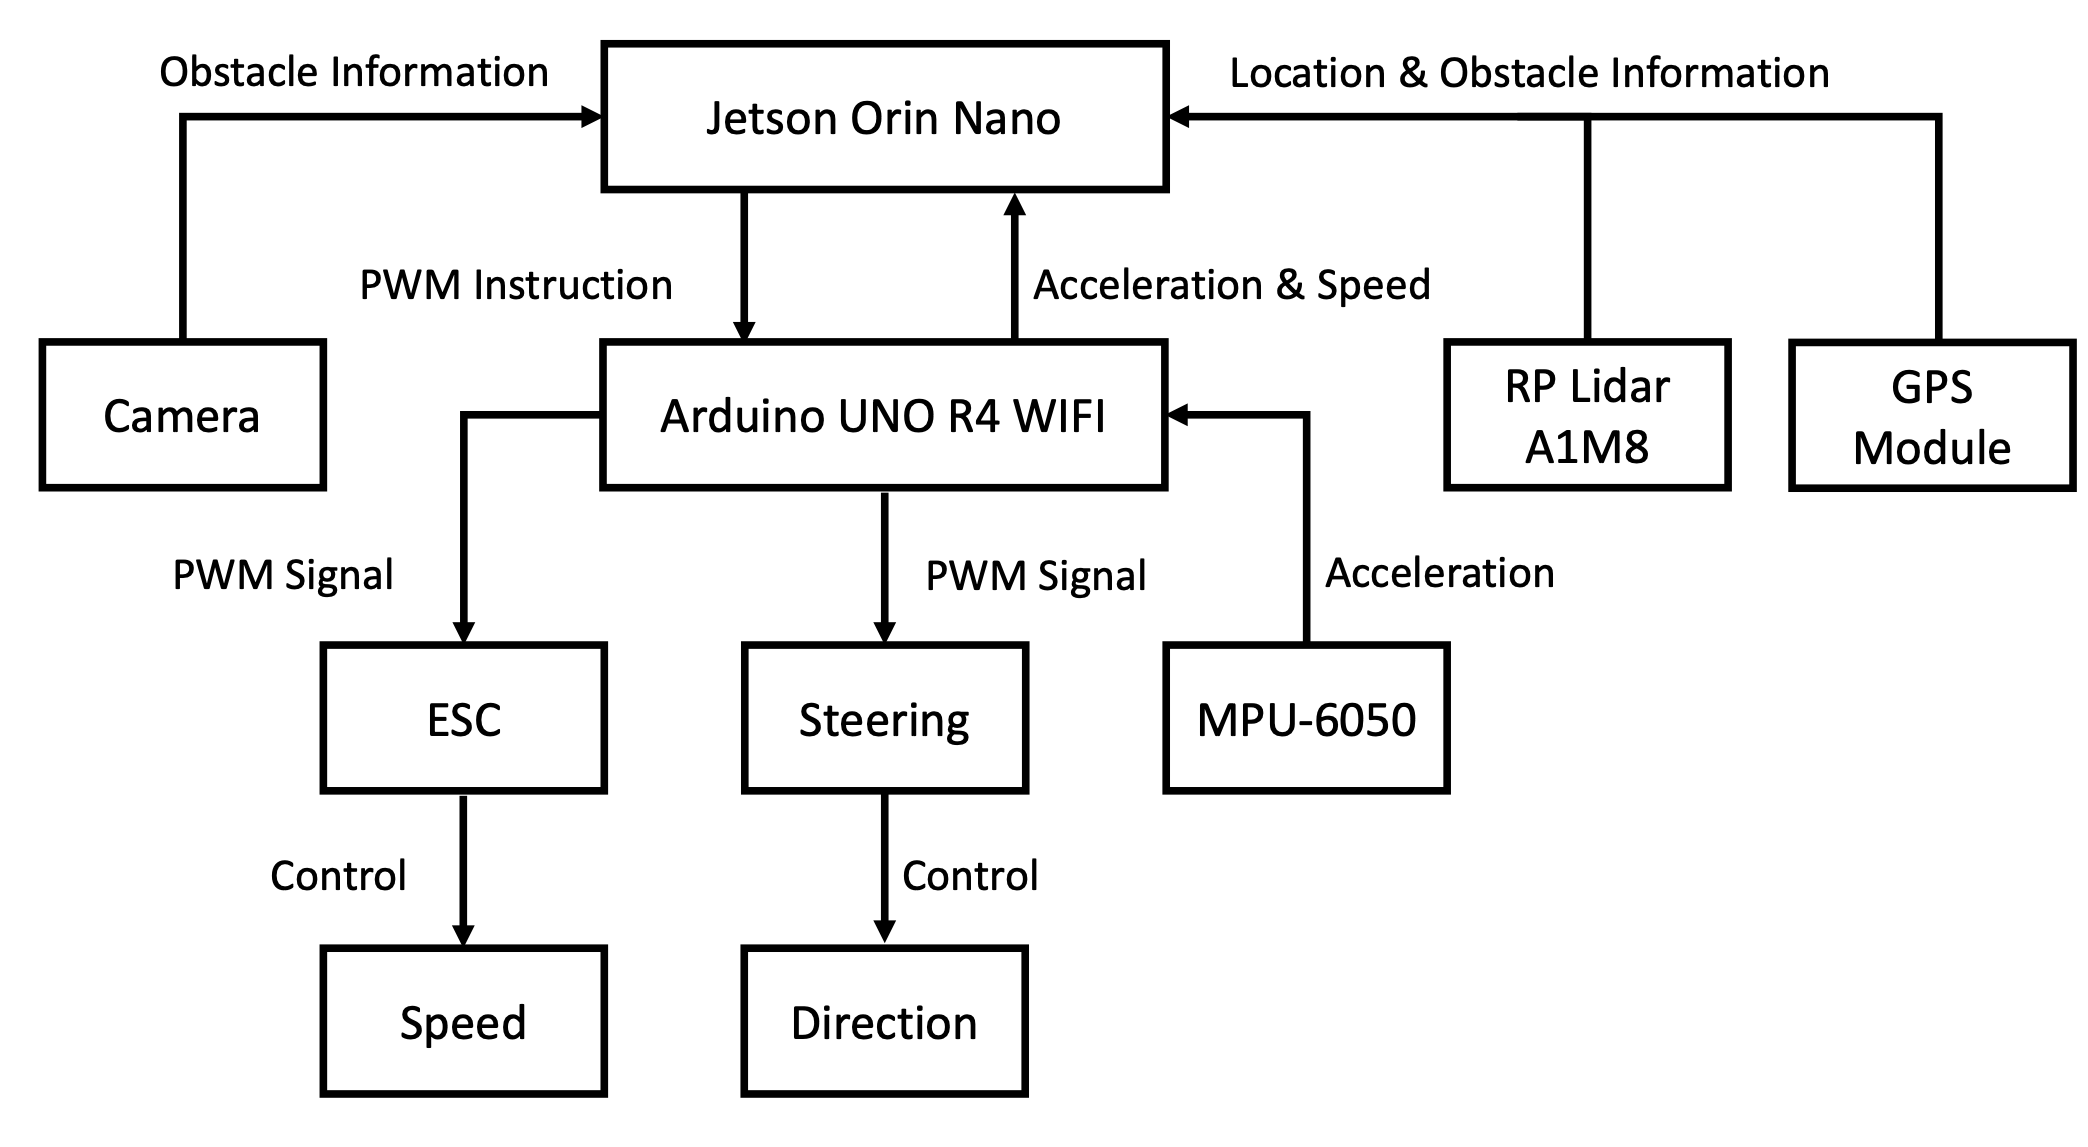
\includegraphics[width=\linewidth]{./images/The Structure of Hardware Part}  % 원본 이미지 경로 유지
    \caption{The Structure of Hardware Part}
    \label{fig:The Structure of Hardware Part}
\end{figure}

Fig~\ref{fig:The Structure of Hardware Part} displays the hardware structure of our solution, divided into 3 parts including Brain, Sensor, and Actuator. Brain includes Jetson Orin Nano as a central controller and Arduino UNO R4 WIFI as a real-time controller. At the early stage, we use Rasphberry Pi4 instead of Jetson Orin Nano for easy and fast development. The sensor includes Camera (Raspberry Pi Camera v2), RPLidar A1M8, MPU-6050, and GPS Module (Spektrum GPS Module). The actuator includes ESC (Electronic Speed Controller) and steering (Servo Motor). These devices are hosted by a RC-Car, along with a 7.2V, 30.24Wh Lipo-power for ESC and steering, and a 5V, 3A powerbank for Jetson Orin Nano. The hardware layout (partly) is shown in Fig.~\ref{fig:hardware}.

\begin{figure}[t]
    \centering
    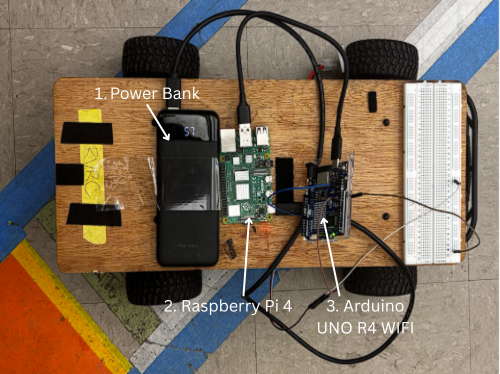
\includegraphics[width=0.75\linewidth]{./images/RC_Car}  % 원본 이미지 경로 유지
    \caption{Hardware platform with labeled components. 1. Power Bank, 2. Raspberry Pi 4, 3. Arduino UNO R4 WIFI}
    \label{fig:hardware}
\end{figure}


% ❌ 겹침 유발 가능성이 큰 음수 간격 제거
% \vspace{-2em}

\vspace{1em}
\subsection{Software Configuration}

\begin{figure}[t]
    \centering
    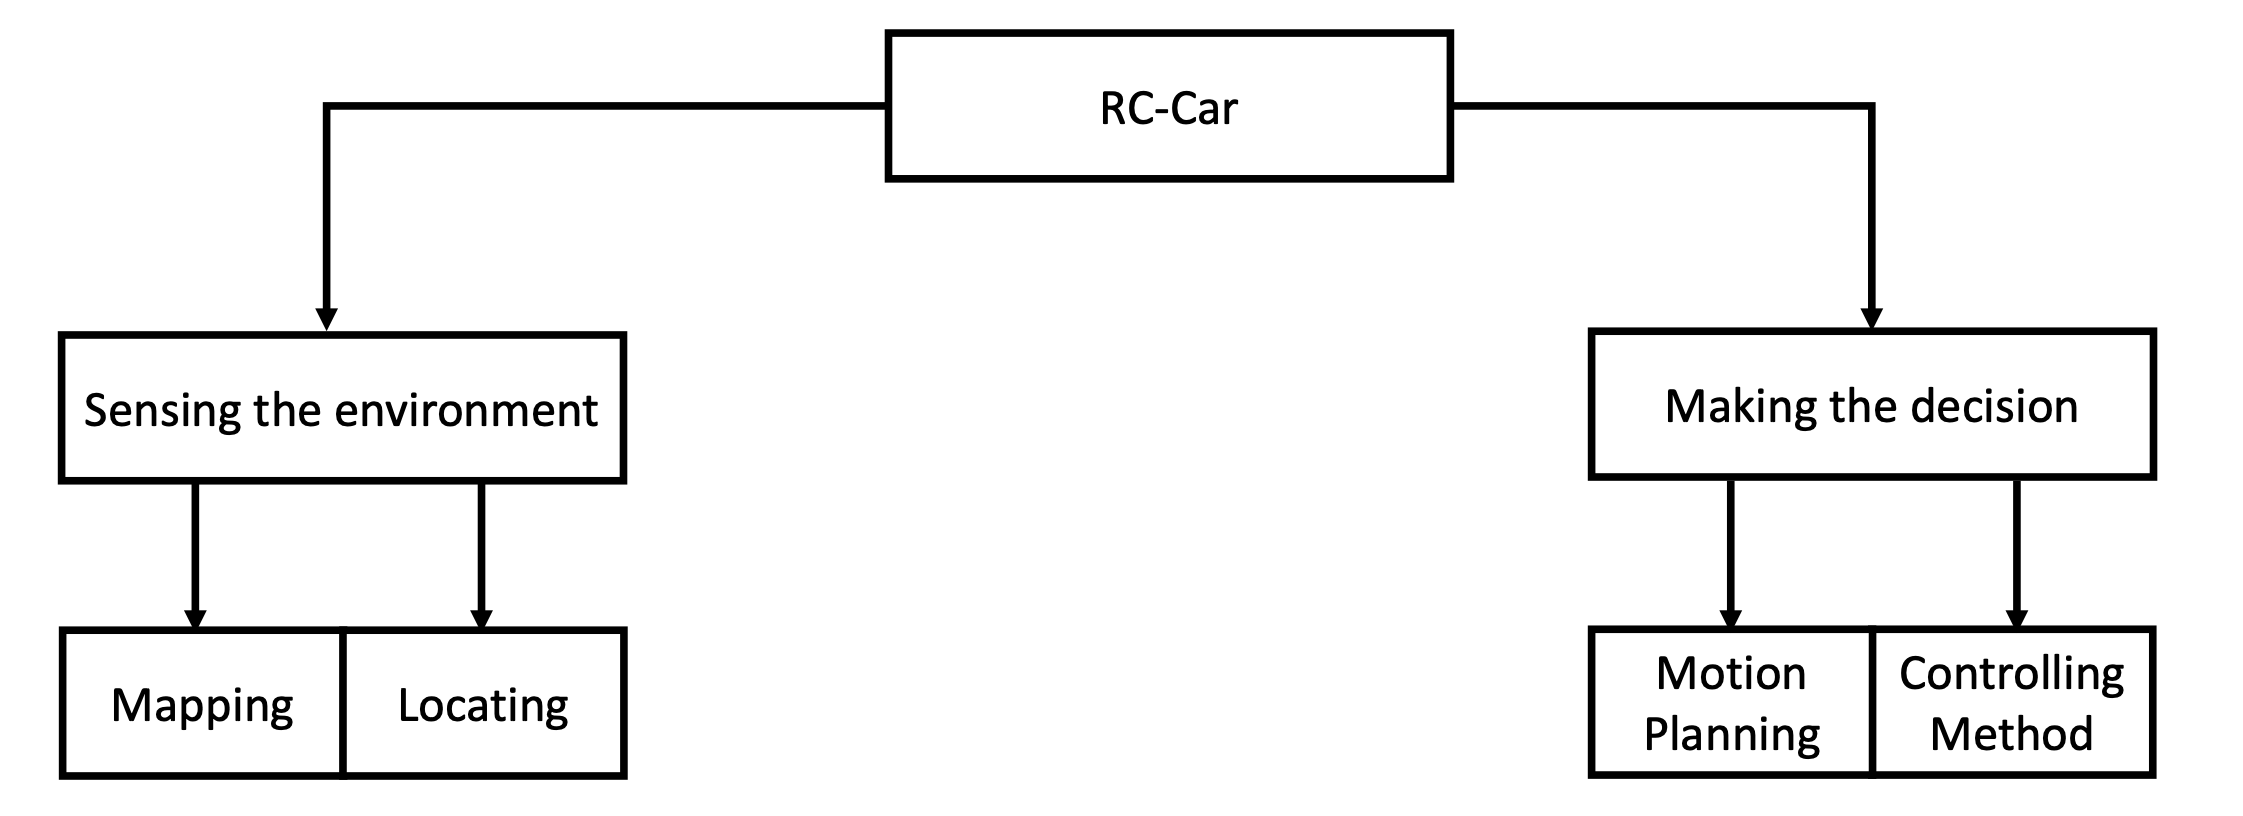
\includegraphics[width=\linewidth]{./images/The Structure of Software Part}  % 원본 이미지 경로 유지
    \caption{The Structure of Software Part}
    \label{fig:The Structure of Software Part}
\end{figure}

Fig~\ref{fig:The Structure of Software Part} displays the software structure of our solution, divided into 2 parts including Sensing the Environment, and Making the Decision. 

For Sensing the Environment, it can be divided into 2 parts including mapping and localization. In the localization module, GPS will provide a coarse-level global position while in the mapping module, OpenStreetMap~\cite{OpenStreetMap} will be deployed to define the overall navigation and route framework. Despite of this, we will also use SLAM~\cite{SLAM} (Simultaneous Localization and Mapping) to get exact real-time mapping and localization and detecting immediate environmental feature. 

For Making the Decision, it can be divided into 2 parts including Motion Planning and Controlling Method. In the Motion Planning module, RRT~\cite{RRT} (Rapidly-exploring Random Tree Algorithm) will be deployed as a basic method with 3 optimization step, including path shortcutting, considering dynamics constrain and real-time update based on SLAM and YOLO~\cite{YOLO} (You Only Look Once). In the Controlling Method module, PID~\cite{PID} (Proportional–Integral–Derivative Controller) will be used in Speed Control and Direction Control. For speed, a dual-loop PID control will be deployed to make sure the start-up and shutdown process is smooth enough. 

The software stack integrates ROS~2 and SLAM for autonomous navigation. ROS~2 serves as middleware to enable modular communication among perception, localization, mapping, planning, and control. Simulation is employed for rapid prototyping, parameter tuning, and evaluation of navigation performance prior to physical deployment.

System-level integration is first validated in simulation. The RC car model is loaded in Gazebo with simulated LiDAR and odometry streams. The \textit{SLAM Toolbox} is employed for real-time mapping and localization: it operates in mapping mode to generate occupancy grids and is subsequently switched to localization-only mode for navigation on prebuilt maps.

Visualization is performed in RViz2, providing real-time monitoring of occupancy grids, robot trajectories, and navigation goals. The Nav2 stack is configured to compute global paths, issue local velocity commands, and execute recovery behaviors using behavior trees. Benchmarking confirms real-time performance on the target platform.

\section{Results}
\label{sec:results}

\subsection{Software Experiment}
The proposed system was implemented and validated in a simulated environment using ROS~2, Gazebo, RViz2, SLAM Toolbox, and Nav2. The experiments demonstrate successful integration of mapping, localization, and autonomous navigation.

\begin{figure}[htbp]
    \thispagestyle{empty} % Removes headers and footers from this page
    \centering
    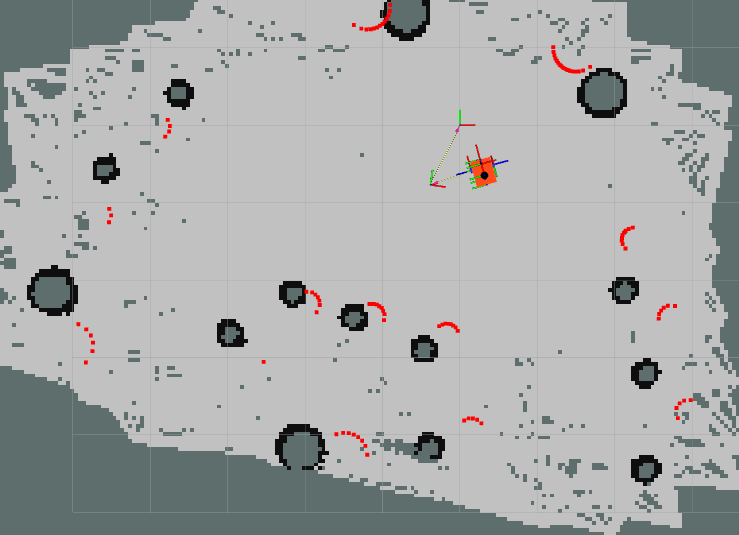
\includegraphics[width=0.4\textwidth,clip]{./images/RVizSLAM_2}
    \caption{RViz2 view of SLAM Toolbox in a simulated environment. The occupancy grid distinguishes free space (white), obstacles (black), and uncertain regions (gray).}
    \label{fig:rvizslam}
\end{figure}

\textbf{~i. Simultaneous Mapping and Localization:} The robot was teleoperated through the simulated world to generate an occupancy-grid map using the asynchronous mode of SLAM Toolbox. As shown in Fig.~\ref{fig:rvizslam}, the mapping resolution was maintained at 0.05~m per cell, enabling accurate delineation of environmental boundaries. A complete map was produced after approximately 3.5~minutes of exploration, and no significant distortions were observed in static scenes.

After switching the SLAM Toolbox configuration to localization mode, the robot accurately localized against the previously serialized map. Pose estimates remained stable during motion with minimal drift, confirming consistent correspondence between simulated sensor data and the global map.

\begin{figure}[htbp]
    \thispagestyle{empty} % Removes headers and footers from this page
    \centering
    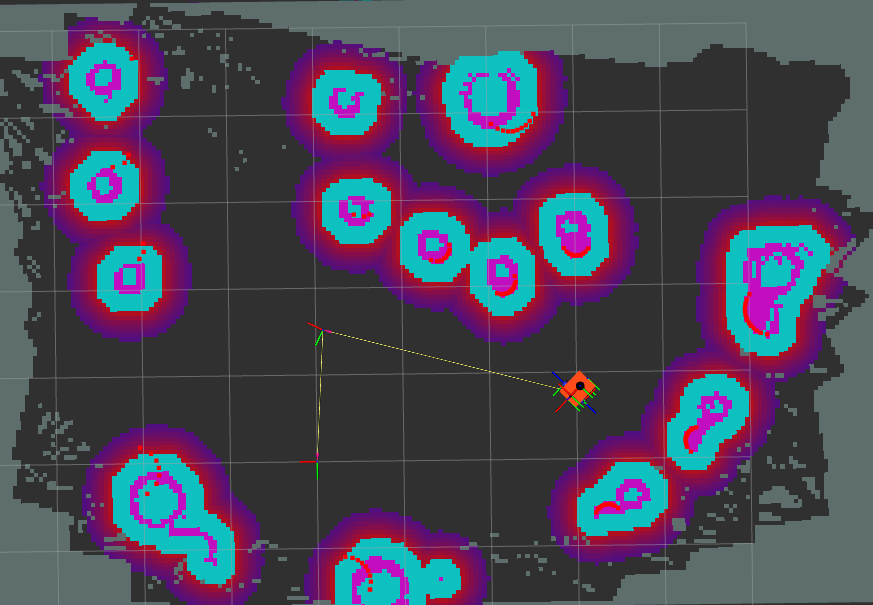
\includegraphics[width=0.4\textwidth,clip]{./images/RVizNav2_2}
    % \vspace{-5}
    \caption{RViz2 visualization of autonomous navigation using the Nav2 stack. Green indicates the planned global path; blue denotes the executed trajectory.}
    \label{fig:rviznav2}
\end{figure}

\textbf{~ii. Autonomous Navigation:} The Nav2 stack was launched to enable autonomous navigation. Global and local costmaps were generated successfully, and navigation goals were assigned through RViz2. As illustrated in Fig.~\ref{fig:rviznav2}, the system produced collision-free paths (green) and executed them smoothly (blue). The robot reached all assigned waypoints with the Performance Metrics in Tab~\ref{Performance Metrics}. 

\begin{table}[h]
\centering
\caption{Performance Metrics}
\begin{tabular}{l l}
\hline
\textbf{Metric} & \textbf{Result} \\
\hline
Mapping time & 3.5 minutes (medium-sized environment) \\
Navigation goal success rate & 100\% (5/5 trials) \\
Average goal completion time & 42.6 seconds \\
Localization drift & negligible in static environments \\
\hline
\end{tabular}
\end{table}

\subsection{Hardware Experiment}
Compared with the software experiments, the hardware implementation started at a later stage. We first focused on achieving stable motion of the vehicle, and subsequently planned to integrate the LiDAR sensor and deploy the SLAM functionality on the hardware platform, with the goal of enabling indoor environment mapping.

\textbf{~i. Smooth start-and-stop motion of the RC-Car:}We successfully enabled the vehicle to perform the start-and-stop process within an indoor environment by using dual-loop PID control method.Specifically, by equipping the vehicle with an IMU module, we obtained data on two key parameters during the start-and-stop process. The measurements were derived from direct acceleration readings and velocity estimation through numerical integration.

\textbf{~ii. Preparatory work for LiDAR-based mapping:}As shown in Fig ~\ref{fig:The Visualization Data from RPLidar}, we operated the RPLidar A1M8 and obtained the corresponding data visualization generated from the LiDAR measurements.Our subsequent work focuses on integrating the SLAM package of ROS2 with the RPLidar to enable real-time mapping capabilities.

\begin{figure}[t]
    \centering
    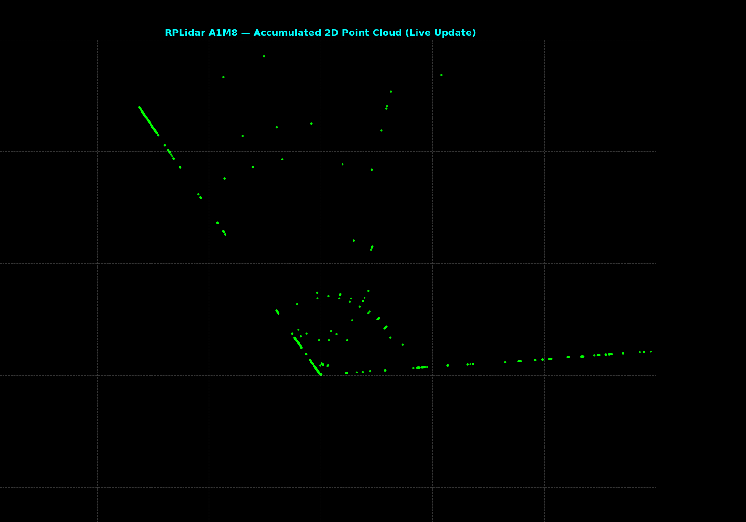
\includegraphics[width=0.75\linewidth]{./images/RPLidar Work}  % 원본 이미지 경로 유지
    \caption{The Visualization Data from RPLidar}
    \label{fig:The Visualization Data from RPLidar}
\end{figure}





\section{Discussion}

\subsection{Analysis of Current Status}
Although numerical results are not yet available, the methodology has been established 
and the system architecture is fully integrated in simulation. 
Planned experiments are expected to confirm that lightweight object detection models can run on embedded hardware 
while supporting SLAM-based navigation in real time.

\subsection{Anticipated Limitations}
Several limitations are anticipated once experiments are conducted:
\begin{itemize}
    \item \textbf{Detection sensitivity:} potential difficulty with small or distant objects.  
    \item \textbf{Lighting robustness:} degraded performance under low-light conditions.  
    \item \textbf{Integration gaps:} challenges in achieving fully autonomous end-to-end operation on hardware.  
\end{itemize}

\subsection{Future Improvements}
Future work will focus on:
\begin{itemize}
    \item Expanding the dataset with low-light and occlusion scenarios for object detection using YOLOv8.
    
    \item Exploring multi-scale models (e.g., YOLOv8 with FPN) for small-object detection.  
    \item Incorporating temporal filtering to reduce false positives.  
    
    \item Executing end-to-end autonomy trials with Nav2 integrated into the hardware platform.  
\end{itemize}

Overall, the midterm stage confirms the feasibility of the proposed framework in principle, 
while highlighting the need for experimental validation and refinement in subsequent phases.


\noindent\textbf{Accomplishments and capability.} Across simulation and hardware, the project delivered a functional end-to-end autonomy pipeline:
(i) LiDAR-based 2D SLAM that maintains consistent occupancy-grid structure when closed-loop speed and yaw feedback is enabled;
(ii) repeatable goal-reaching with Nav2 without collisions on a small indoor track; and
(iii) a working vision-cue pathway (YOLO) that is ready for tighter coupling with navigation.
These results establish a robust baseline under low-cost compute and hobby-grade actuation, and clarify the current capability level of the system.

% \newpage
\section*{CRediT Author Statement}
\small
All authors contributed equally as collaborators and shared responsibility throughout the project.  
Each author played a primary role while also supporting other aspects of the work as part of a horizontal and cooperative team effort.

\begin{itemize}
    \item \textbf{SangWoo Park:} Conceptualization, Hardware Integration, Methodology, Visualization, Writing : Original Draft, Cross-Team Coordination  
    \item \textbf{Hantao Fu:} Software Development, Validation, Formal Analysis, Writing : Review \& Editing  
    \item \textbf{Mehul Goel:} Software Development, Data Curation, Experimental Investigation, Testing, Visualization, Writing : Review \& Editing  
\end{itemize}

All authors participated in discussions, reviewed the manuscript, and approved the final version for publication.

\normalsize

\section*{Acknowledgment}
\small
The authors would like to express their sincere gratitude to Professor Yu Kee Ooi and Professor Joseph Young for their continuous guidance, technical insights, and encouragement throughout the project.  
We also extend our appreciation to the teaching





\begin{thebibliography}{00}

\bibitem{cairo_rc}
F.~Mahmoud, ``Autonomous RC-Car,'' GitHub repository, 2025. [Online]. Available: \url{https://github.com/farah-mahmoud/Autonomous-RC-Car}

\bibitem{donkeycar}
Donkey Car Project, ``Create an Autopilot,'' GitHub repository, 2025. [Online]. Available: \url{https://github.com/autorope/donkeycar}

\bibitem{f1tenth}
ECE UCSB, ``F1TENTH Project,'' 2024. [Online]. Available: \url{https://courses.ece.ucsb.edu/ECE188/188_F24Ilan/Projects%20Offered/F1TENTH_2024-25.pdf}

\bibitem{mit_racecar}
MIT Racecar Project, ``Racecar\_Gazebo,'' GitHub repository, 2025. [Online]. Available: \url{https://github.com/mit-racecar/racecar_gazebo}

\bibitem{pmlr}
Proceedings of Machine Learning Research, ``Workshop and Conference Proceedings,'' 2025. [Online]. Available: \url{https://proceedings.mlr.press/}

\bibitem{smartcam_book}
Autonomous RC Car GP Book, Chapter 3--4, 2025.

\bibitem{OpenStreetMap}
M. Haklay and P. Weber, "OpenStreetMap: User-Generated Street Maps," in IEEE Pervasive Computing, vol. 7, no. 4, pp. 12-18, Oct.-Dec. 2008, doi: 10.1109/MPRV.2008.80.

\bibitem{SLAM}
H. Durrant-Whyte and T. Bailey, "Simultaneous localization and mapping: part I," in IEEE Robotics \& Automation Magazine, vol. 13, no. 2, pp. 99-110, June 2006, doi: 10.1109/MRA.2006.1638022.

\bibitem{RRT}
LaValle, Steven. "Rapidly-exploring random trees: A new tool for path planning." Research Report 9811 (1998).

\bibitem{YOLO}
Redmon, Joseph, et al. "You only look once: Unified, real-time object detection." Proceedings of the IEEE conference on computer vision and pattern recognition. 2016.

\bibitem{PID}
Borase, Rakesh P., et al. "A review of PID control, tuning methods and applications." International Journal of Dynamics and Control 9.2 (2021): 818-827.





\end{thebibliography}
% \bibitem{FSD}
% Tesla, \emph{Autopilot and Full Self-Driving (Supervised)}\hskip 1em plus 0.5em minus 0.4em\relax Tesla

% \bibitem{Autopilot}
% K. Nived Maanyu, \emph{A Study on Tesla Autopilot}\hskip 1em plus 0.5em minus 0.4em\relax Sreenidhi Institute of Science And Technology, 2020 

% \bibitem{ExSolution}
% Syazvinski, \emph{Traffic-Light-Detection-Color-Classification}\hskip 1em plus
% 0.5em minus 0.4em\relax GitHub repository, 2023.
% [Online]

% \bibitem[Fig.4]
% *Carousel, \emph{Manderfield Highway Information}\hskip 1em plus 0.5em minus 0.4em\relax Beaver County, 2024

% \bibitem[Fig.5-(a)]
% *Kidloverz22, \emph{Seoul,South Korea-March 2019: Close up image of traffic light changes color with Korean traffic street sign}\hskip 1em plus 0.5em minus 0.4em\relax Dreamstime.com

% \bibitem[Fig.5-(b)]
% *Katherine Tweed, \emph{Better Traffic Light Simulations Could Cut Travel Time and Gas Use}c IEEE Spectrum, 2014
% \bibitem[Fig.5-(c)]
% *Ben Watanabe, \emph{Those blue lights on traffic signals help nab red-light runners}\hskip 1em plus 0.5em minus 0.4em\relax HeraldNet, 2022





% biography section
% 
% If you have an EPS/PDF photo (graphicx package needed) extra braces are
% needed around the contents of the optional argument to biography to prevent
% the LaTeX parser from getting confused when it sees the complicated
% \includegraphics command within an optional argument. (You could create
% your own custom macro containing the \includegraphics command to make things
% simpler here.)
%\begin{IEEEbiography}[{\includegraphics[width=1in,height=1.25in,clip,keepaspectratio]{mshell}}]{Michael Shell}
% or if you just want to reserve a space for a photo:


% insert where needed to balance the two columns on the last page with
% biographies
%\newpage


% You can push biographies down or up by placing
% a \vfill before or after them. The appropriate
% use of \vfill depends on what kind of text is
% on the last page and whether or not the columns
% are being equalized.

%\vfill

% Can be used to pull up biographies so that the bottom of the last one
% is flush with the other column.
%\enlargethispage{-5in}



% that's all folks
\end{document}


